\chapter{Calculation of Grating Ratio}\label{GratingRatioAppendix}
In order to narrow the linewidth of the master laser and make it more tunable and stable, we have mounted a diffraction grating in a Littrow configuration. The gratings are mounted on piezoelectric actuators that can be automatically moved in unison by our control circuitry. 

However, in order for this to work, it is important to verify that the piezos can be scanned in such a way that the resonances of the external cavity track smoothly. In order to accomplish this, one must find a ratio that relates the relative rates at which each piezoelectric actuator is scanned. 

Normally, this is not very tricky. However, at one point we discovered that for certain geometries, the appropriate ratio might be negative. To this end, we created the following Mathematica notebook to model the motion of the grating and help us to ensure that our electronics are capable of moving the actuators properly. 
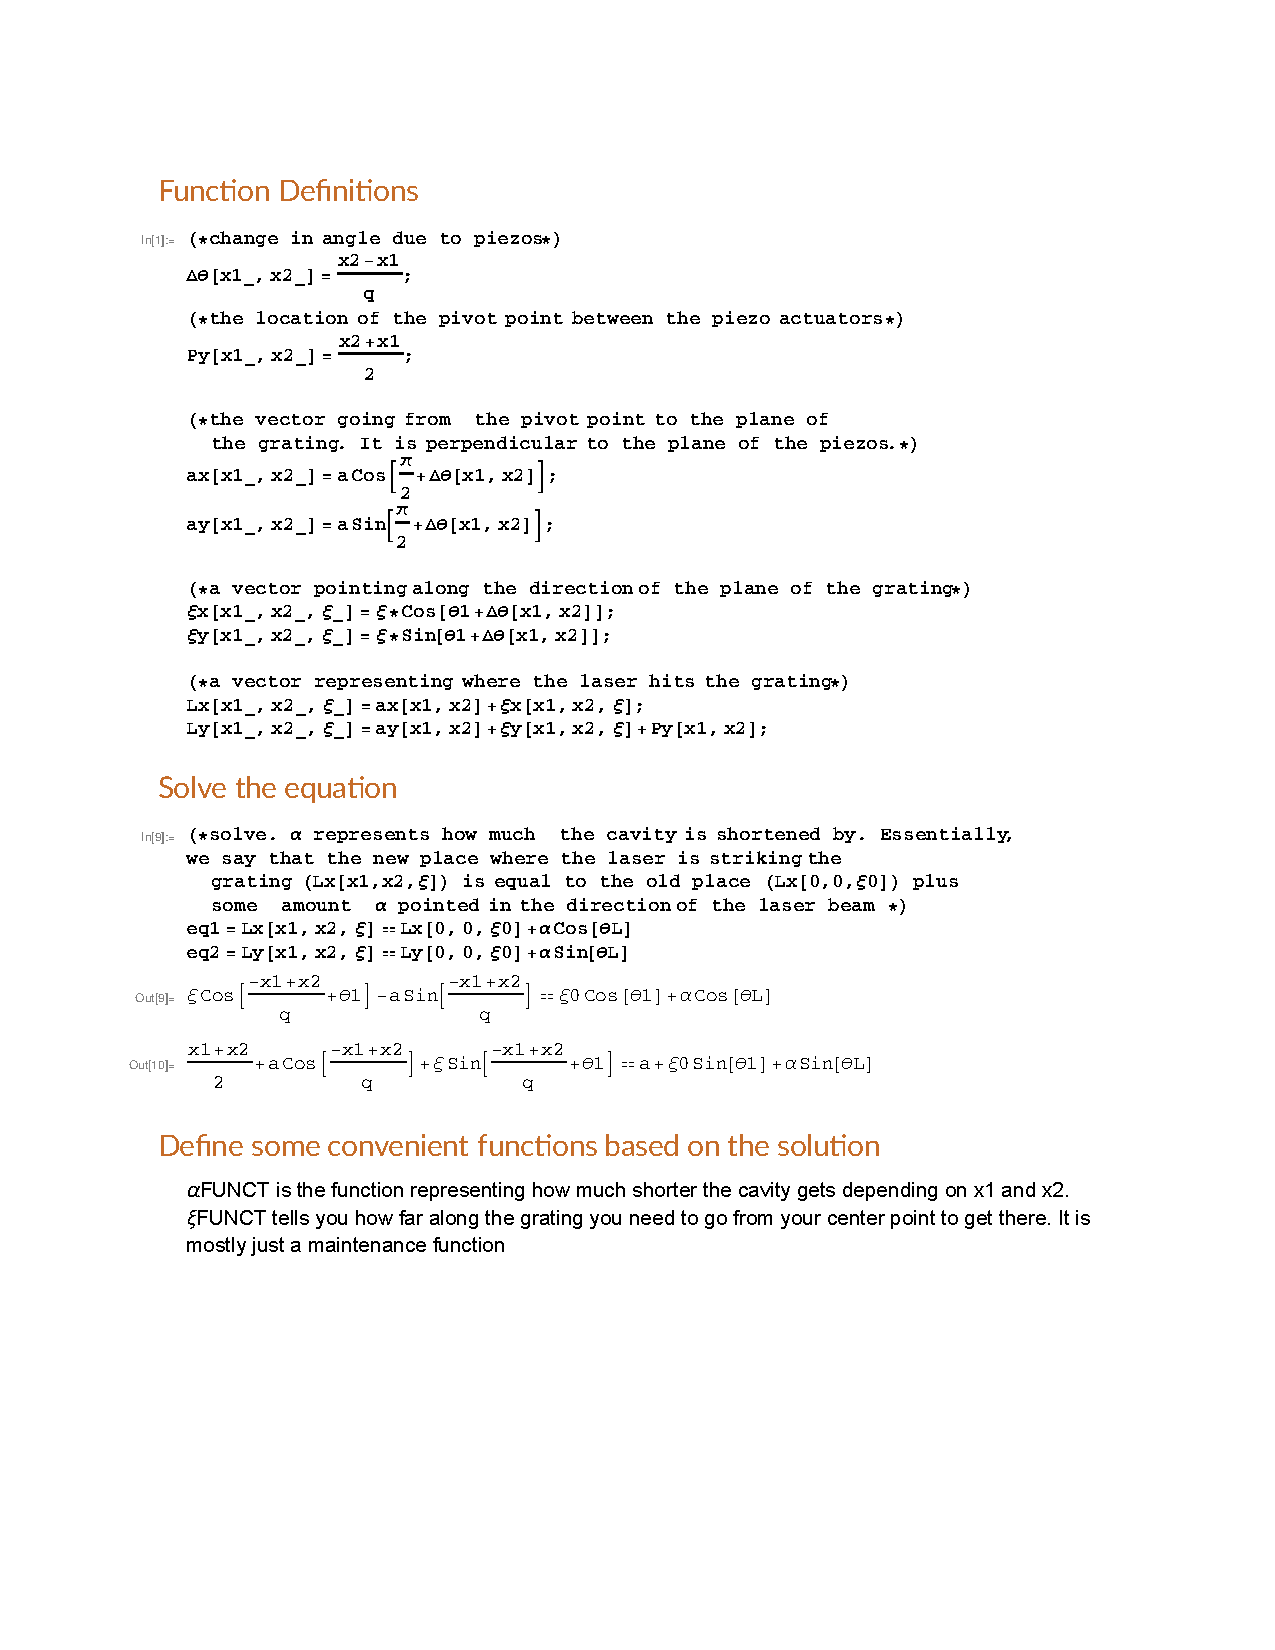
\includepdf[pages={1-10}]{grating_motion}


